\begin{figure*}[htb]
  \centering
  \begin{subfigure}[t]{0.32\textwidth}
    \centering
    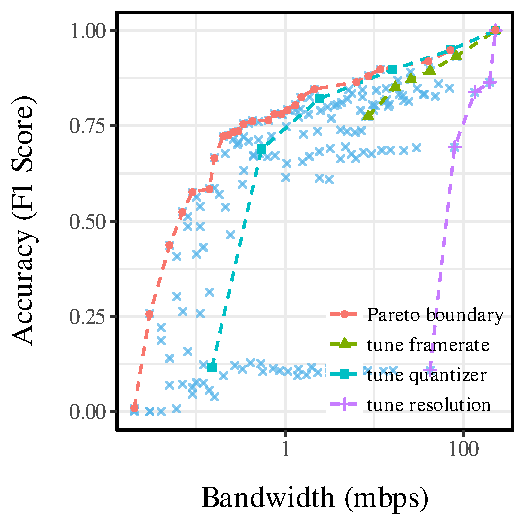
\includegraphics[width=\textwidth]{figures/profile-mot.pdf}
    \caption{Pedestrian Detection (PD)}
    \label{fig:pd-profile}
  \end{subfigure}
  \hfill
  \begin{subfigure}[t]{0.32\textwidth}
    \centering
    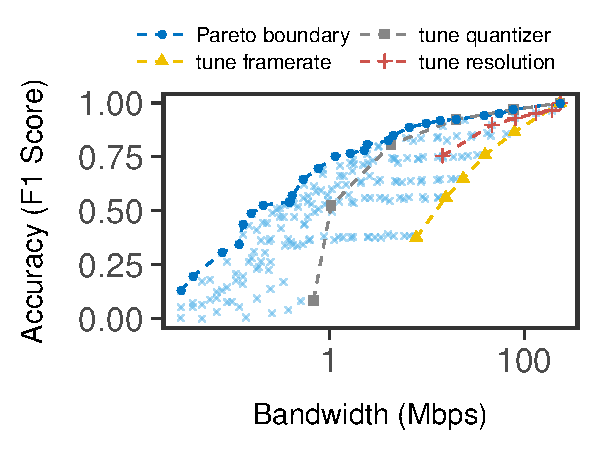
\includegraphics[width=\textwidth]{figures/profile-darknet.pdf}
    \caption{Augmented Reality (AR)}
    \label{fig:ar-profile}
  \end{subfigure}
  \hfill
  \begin{subfigure}[t]{0.32\textwidth}
    \centering
    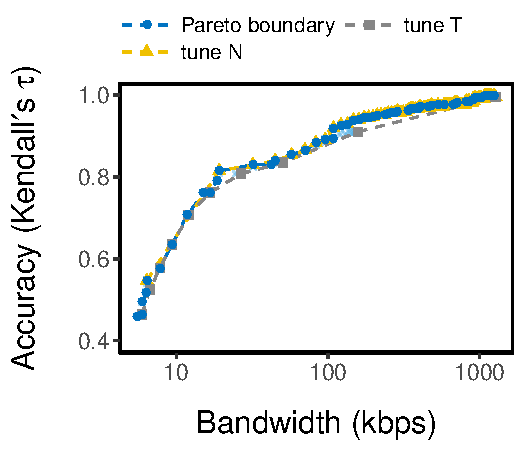
\includegraphics[width=\textwidth]{figures/profile-topk.pdf}
    \caption{Top-K (TK)}
    \label{fig:tk-profile}
  \end{subfigure}
  \caption{Application profiles of three applications. Each cross point is one
    configuration $c$'s performance $(B(c), A(c))$. All figures show the Pareto
    boundary as well as the performance if only tuning one dimension. Note the
    x-axis is in log scale.}
  \label{fig:all-profiles}
\end{figure*}

\section{Evaluation}
\label{sec:evaluation}

In this section, we show the evaluations of \sysname{}, summarizing the results
as follows.

\begin{itemize}
\item[\autoref{sec:application-profiles}] \sysname{} generates Pareto-optimal
  profiles across multiple dimensions with precision
  (\autoref{fig:all-profiles}).
\item[\autoref{sec:online-profiling}] Our parallel and sampling profiling speeds
  up offline and online profiling (\autoref{fig:parallel},
  \autoref{fig:online-tricks}).
\item[\autoref{sec:runtime-adaptation}] At runtime, \sysname{} applications
  achieve sub-second latency and nominal accuracy drop
  (\autoref{fig:all-runtime}).
\item[\autoref{sec:multi-task-alloc}] \sysname{} profiles allow different
  resource allocations, such as utility fairness (\autoref{fig:multitask}).
\end{itemize}

\subsection{Application Profiles}
\label{sec:application-profiles}

We run our offline profiling using the training dataset described
in~\autoref{tab:apps}.  \autoref{fig:all-profiles} shows the learned
profiles. In each figure, the cross dots represent the bandwidth demand and
application accuracy of one configuration. We highlight the Pareto-optimal
boundary $\mathbb{P}$ with blue dashed lines. To understand each dimension's
impact on the degradation, we highlight configurations from tuning only
\textit{one} dimension. From these profiles, we make the following observations:

\para{Large bandwidth variation.} For all three applications, their bandwidth
requirements have two to three orders of magnitude of difference (note the
x-axis is in log scale). For PD and AR, the most expensive configuration
transmits videos at 1920x1080, 30 FPS and 0 quantization; it consumes 230 mbps. In
constrast to the large bandwidth variation, there is a smaller variation in
accuracy. In PD, for example, even after the bandwidth reduces to 1 mbps (less
than 1\% of the maximum), the accuracy is still above 75\%. This allows
\sysname{} applications to operate at a high accuracy configuration even under
severe network deterioration.

\para{Multiple dimensions achieve the optimal.} Comparing dashed lines in each
profile, we see that the Pareto-optimal configurations are only achievable when
multiple knobs are in effect. Tuning only one dimension often leads to
sub-optimal performance. Although Top-K's Pareto-optimal boundary aligns with
the performance of tuning \texttt{N}, i.e.\,tuning \texttt{T} doesn't contribute
much for this dataset, for another dataset with a different distribution,
the behavior will probably change.

\para{Each dimension affects differently}. Within a single profile, the
difference between tuning individual dimensions is evident. For PD, tuning
resolution (the red line) leads to a quicker accuracy drop in comparison to
tuning the frame rate (the yellow line). Comparing PD and AR, the same dimension
has different impact. Tuning resolution is less harmful in AR than PD; while
tuning frame rate hurts AR more than PD\@. This echoes our initial observation
in~\autoref{sec:making-case-sys-approach} that application- and context-specific
optimizations don't generalize.

\para{Quantification with precision}. The generated profiles are actionable
configurations that control the knobs with precision. For example,
if PD transmits video at 1920x1080 resolution, \(10~\text{FPS}\) and
a quantization of 20, it will consume 11.7 mbps of bandwidth, achieving roughly
90\% accuracy. This saves developers from laboriously analyzing their
application to compute manual policies.

\subsection{Profiling Efficiency and Online Profiling}
\label{sec:online-profiling}

This section focuses on the AR application as a case study;
our profiling techniques---parallelism and sampling---do not make assumptions about the application; therefore, the evaluation results can be generalized to other applications.

AR allows 216 different configurations: 6 resolutions, 6 frame rates and 6
quantization levels. Processing a frame with YOLO~\cite{redmon2016yolo9000} on
GeForce\textregistered\space GTX 970 takes roughly 30 ms.\footnote{YOLO resizes
  an input image to a fixed neural network size. Evaluating all images (with
  different resolutions) takes a similar amount of time.} But different
configurations require different amounts of processing. For example, a \(10~\text{FPS}\)
video has 1/3 of the frames to process in comparison to a \(30~\text{FPS}\) video.
In our experiment, to evaluate all 216 configurations, it takes 52 seconds for 1-second
worth of data. We denote such overhead as 52X\@. \autoref{sec:automatic-profiling} discusses techniques to improve the
profiling efficiency; we present their evaluations as follows.

\begin{figure}
  \centering
  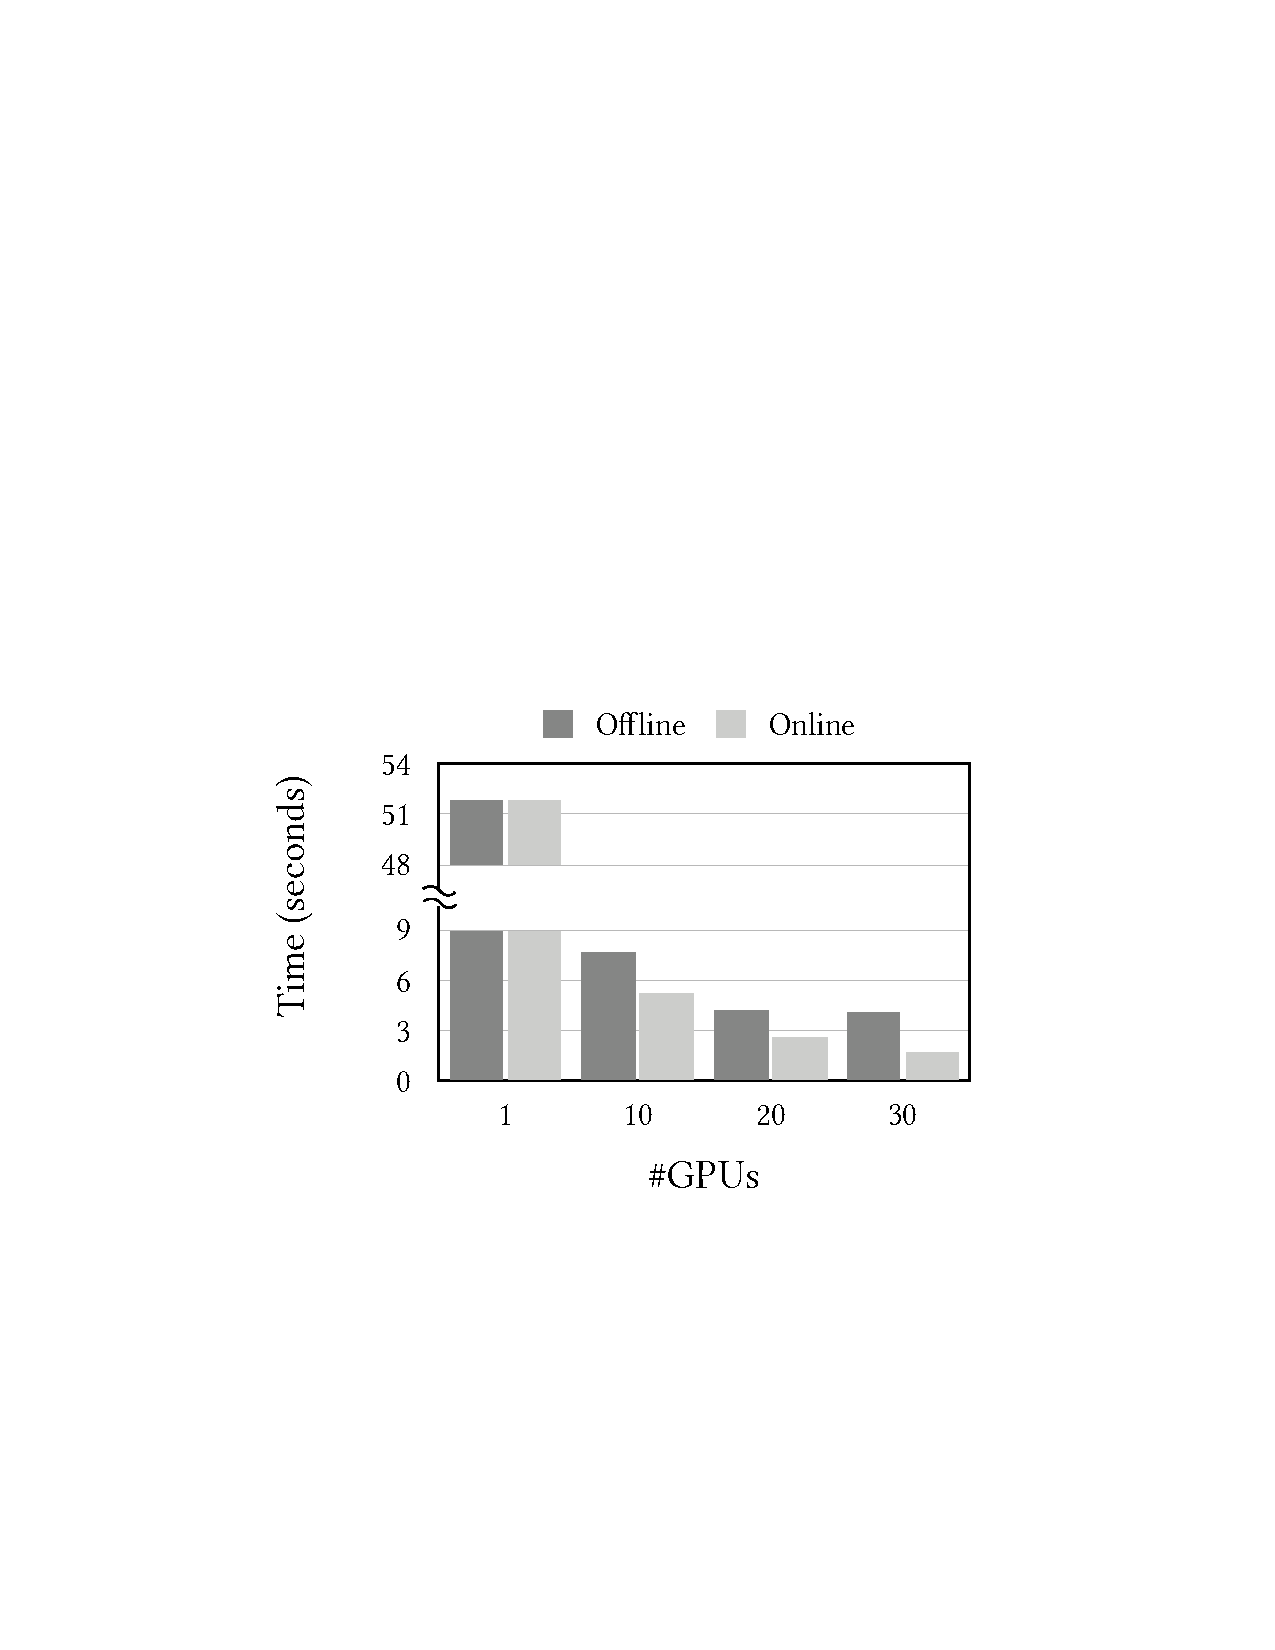
\includegraphics[width=0.9\columnwidth]{figures/parallel.pdf}
  \caption{Parallelism speeds up both offline and online profiling.
  The y-axis shows the profiling time for 1-second video.}
  \label{fig:parallel}
\end{figure}

\para{Parallelism reduces the profiling time (\autoref{fig:parallel})}. Because
evaluating each individual configuration is independent of other configurations,
we parallelize the profiling task by assigning configurations to GPUs.
$(i)$~Our offline profiling assigns configurations randomly.
With the increased number of GPUs, the overhead reduces from 52X to 4X with 30 GPUs.
$(ii)$~Our online profiling assigns configurations based on the processing times collected during offline.
\sysname{} currently uses LPT assignment and can reduce the overhead to 1.75X with 30 GPUs.

\para{Sampling techniques speed up online profiling (\autoref{fig:online-tricks}).}
Before we evaluate the speed up, we validate
\textit{model drifts} with real-world data. We use the profile
trained in an office environment.
According to the profile, the application should operate at a configuration of 1280x720 resolution, 30 FPS and a quantization of 20 to meet 11 mbps available bandwidth.
We test it against a home environment, and at about t=100s, the camera points out
of the window to detect objects on the street. Because of the scene change, the
configuration fails to predict runtime bandwidth, as illustrated in
\autoref{fig:offline}.

To correct the profile, if we continuously run the profiling online and update
the profile, the application will choose the right configuration to meet the bandwidth limit.
\autoref{fig:online} shows the bandwidth prediction when we continuously
profile with the past 30 seconds of video. At time t=120s, the new
prediction corrects the drifts. The downside of continuous profiling, as
discussed earlier, is the cost: 52X overhead with 1 GPU\@. In addition to
parallelism, \sysname{} uses two other techniques for online profiling
(improvements in \autoref{tab:online}):

(i) Partial data: Instead of using all the past data, we run profiling with only
a fraction of the raw data.
\autoref{fig:online-partial} shows the bandwidth prediction if we only use 10
seconds of data out of the past 30 seconds. In this way, although the profile
may be less accurate (the mis-prediction at t=80--100s), and there is a
delay in reacting to data change (the mis-prediction is corrected after t=125s), we save the online profiling by 3$\times$ (from 52X to 17X).

(ii) Partial configurations: If we use the past profile as a reference and only
measure a subset of all Pareto-optimal configurations, the savings can be
substantial. A full profiling is only triggered if there is a significant
difference. \autoref{fig:online-trigger} shows the bandwidth prediction if we
evaluate 5 configurations continuously and trigger a full profiling when the
bandwidth estimation is off by 1 mbps or the accuracy is off by 10\%.
For our test data, this scheme is enough to correct model drifts by predicting an accurate bandwidth usage
(compare \autoref{fig:online} and \autoref{fig:online-trigger}).
The overhead reduces to 6X because we run full profiling less often (only two times in this experiment).

When we combine the parallelization and sampling-based profiling, we can further
reduce the profiling overhead. For example, scheduling five GPUs running 5
configurations continuously to check for model drifts will reduce the overhead
to 1X\@. In practice, the amount of resources to use will depend on the budget and the importance
of the job.

\begin{figure}
  \centering
  \begin{subfigure}[t]{0.48\columnwidth}
    \centering
    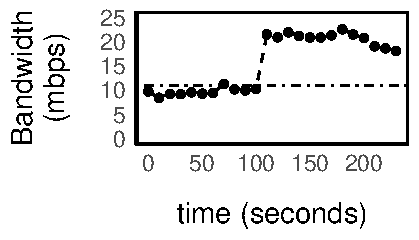
\includegraphics[width=\textwidth]{figures/online1.pdf}
    \caption{Offline only}
    \label{fig:offline}
  \end{subfigure}
  \hfill
  \begin{subfigure}[t]{0.48\columnwidth}
    \centering
    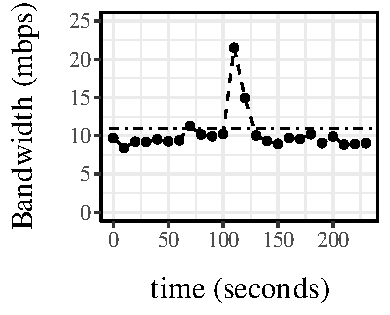
\includegraphics[width=\textwidth]{figures/online2.pdf}
    \caption{Online (continuous)}
    \label{fig:online}
  \end{subfigure}
  \\
  \vspace{1.5em}
  \begin{subfigure}[t]{0.49\columnwidth}
    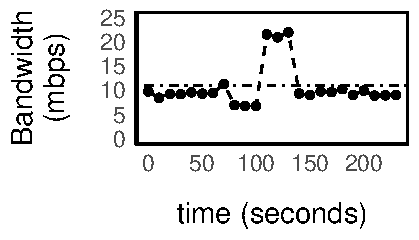
\includegraphics[width=\textwidth]{figures/online3.pdf}
    \caption{Partial data}
    \label{fig:online-partial}
  \end{subfigure}
  \hfill
  \begin{subfigure}[t]{0.49\columnwidth}
    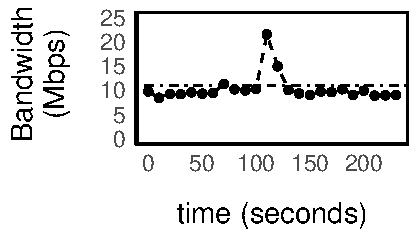
\includegraphics[width=\textwidth]{figures/online4.pdf}
    \caption{Partial configurations}
    \label{fig:online-trigger}
  \end{subfigure}
  \caption{The horizontal reference line is the target bandwidth (11 mbps). We omit accuracy predictions  since in all schemes they are similarly high (\textasciitilde 90\%). (1) Online profiling is necessary to handle model drifts ((a) vs.\,(b-d)). (2) Sampling techniques---partial data (c) and partial configurations (d)---can correct model drifts with less profiling overhead (see \autoref{tab:online}), compared to continuous (b).}
  \label{fig:online-tricks}
\end{figure}

%% Offline: 0
%% Online: 1 frame (1852.21 GPU * seconds)
%% Online (1/10)   (185.2 GPU * seconds)
%% Trigger         ( GPU * seconds)

\begin{table}[t]
  \centering
  \begin{tabular}{c c c}
    \toprule
    online scheme & overhead & improvements \\
    \midrule
    continuous & 52X & baseline \\
    partial data & 17X & 3$\times$\\
    partial configurations & 6X & 8.7$\times$ \\
    \bottomrule
  \end{tabular}
  \caption{Sampling techniques speed up the profiling. We use X to denote the overhead of processing one-second worth of data; and $\times$ for the improvements.}
  \label{tab:online}
\end{table}

%% Note that it is not always needed to do online profiling. PD's test data doesn't exhibit model drift.
%% Nor is online profiling always expensive. Processing TK over all configurations.

\begin{figure*}
  \begin{subfigure}{\linewidth}
    \centering
    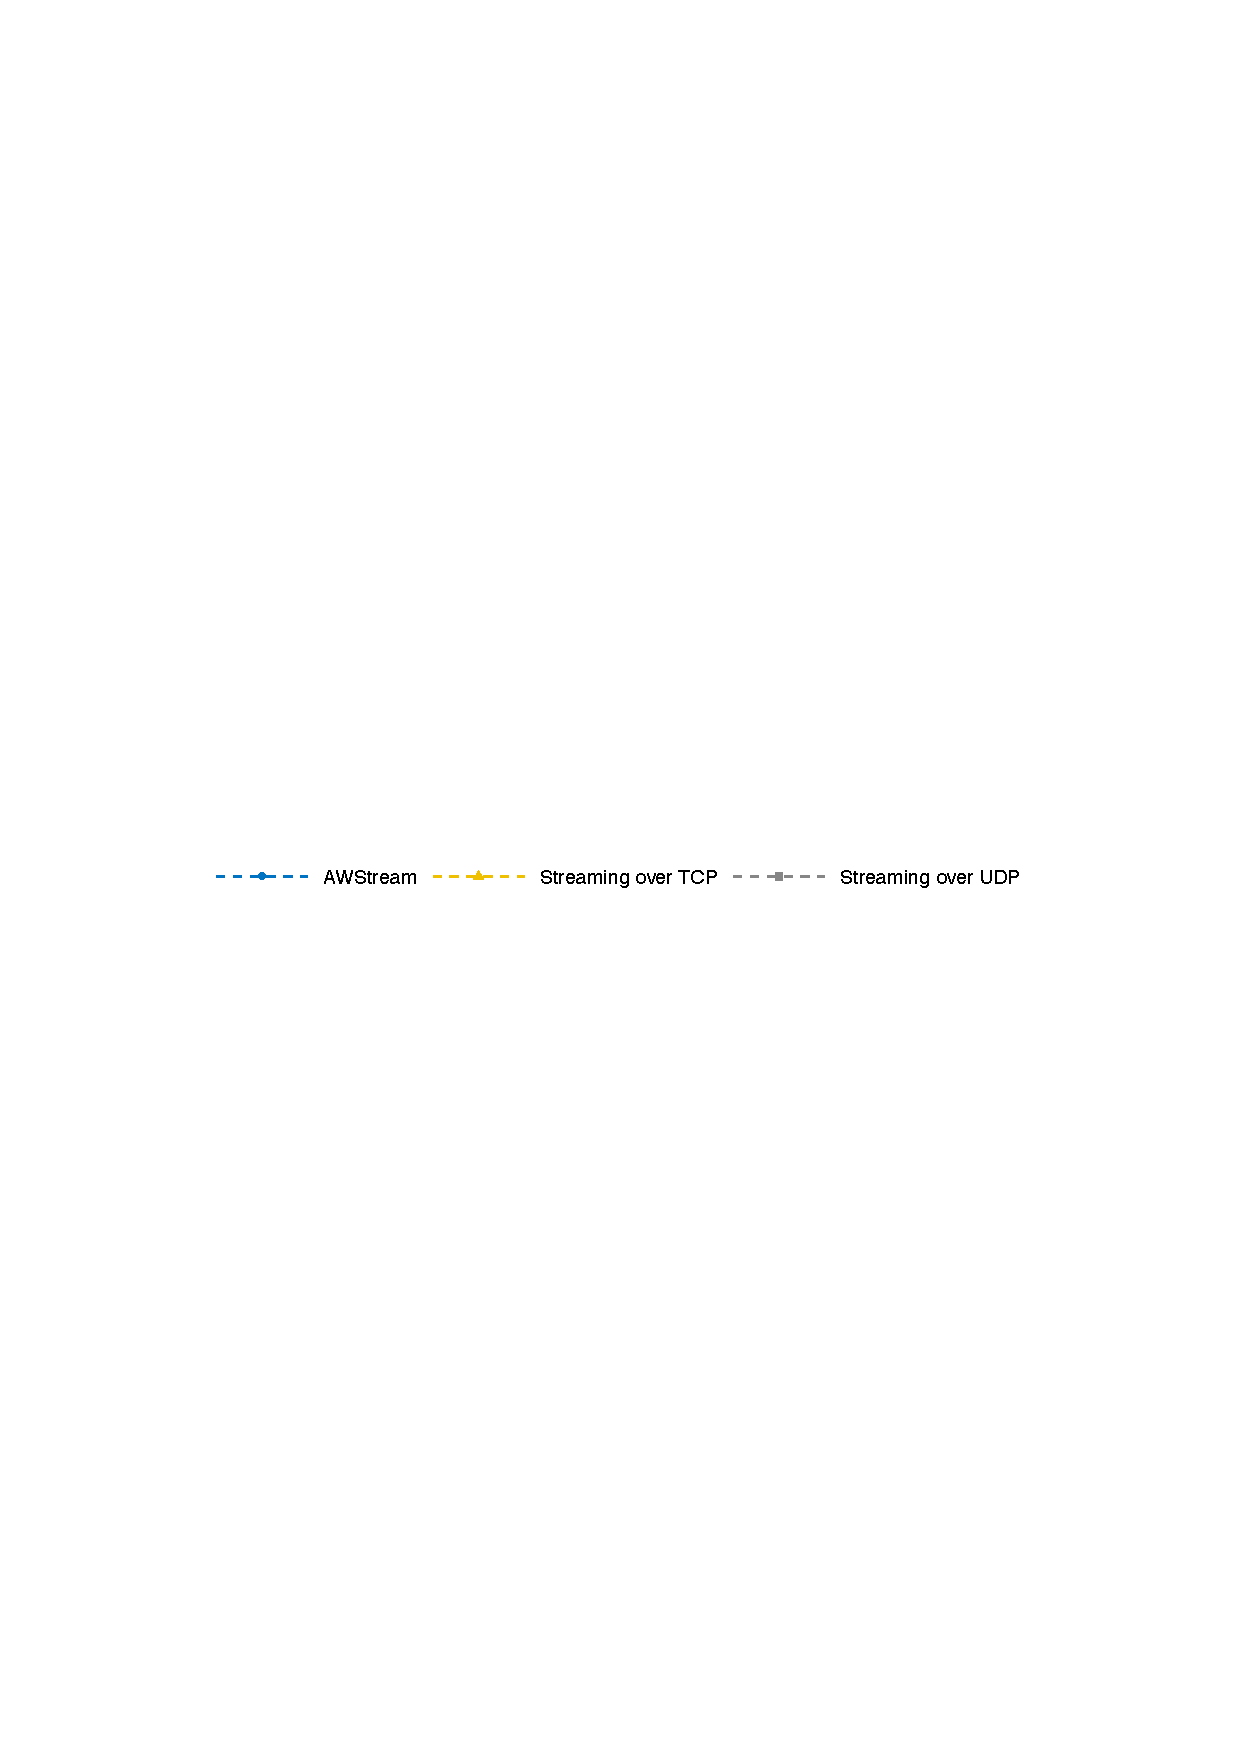
\includegraphics[width=0.5\columnwidth]{figures/runtime-legend.pdf}
  \end{subfigure}
  \\
  \vspace{0.4em}
  \begin{subfigure}{0.3\textwidth}
    \centering
    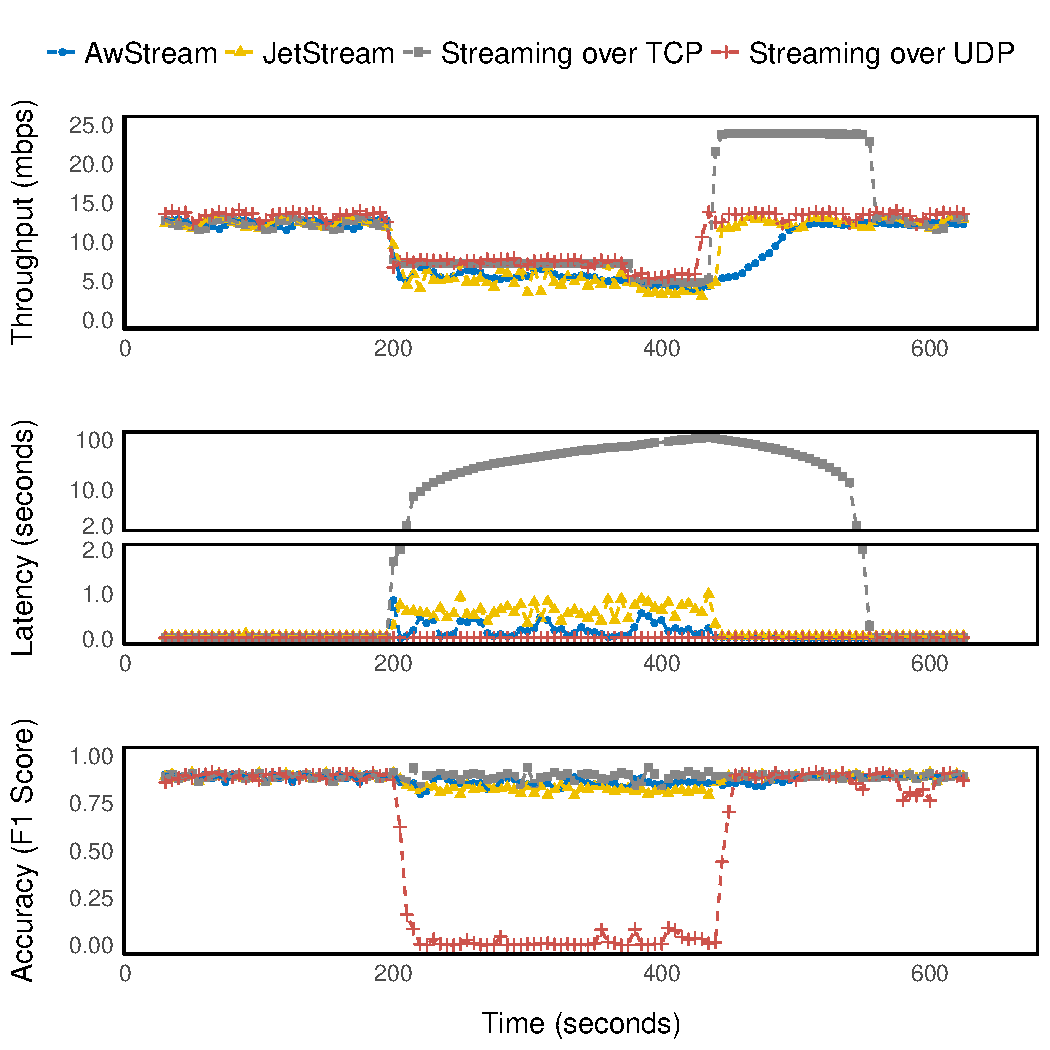
\includegraphics[width=\textwidth]{figures/runtime-mot-verticle.pdf}
    \caption{Pedestrian Detection (PD)}
    \label{fig:pd-runtime}
  \end{subfigure}
  \hfill
  \begin{subfigure}{0.3\textwidth}
    \centering
    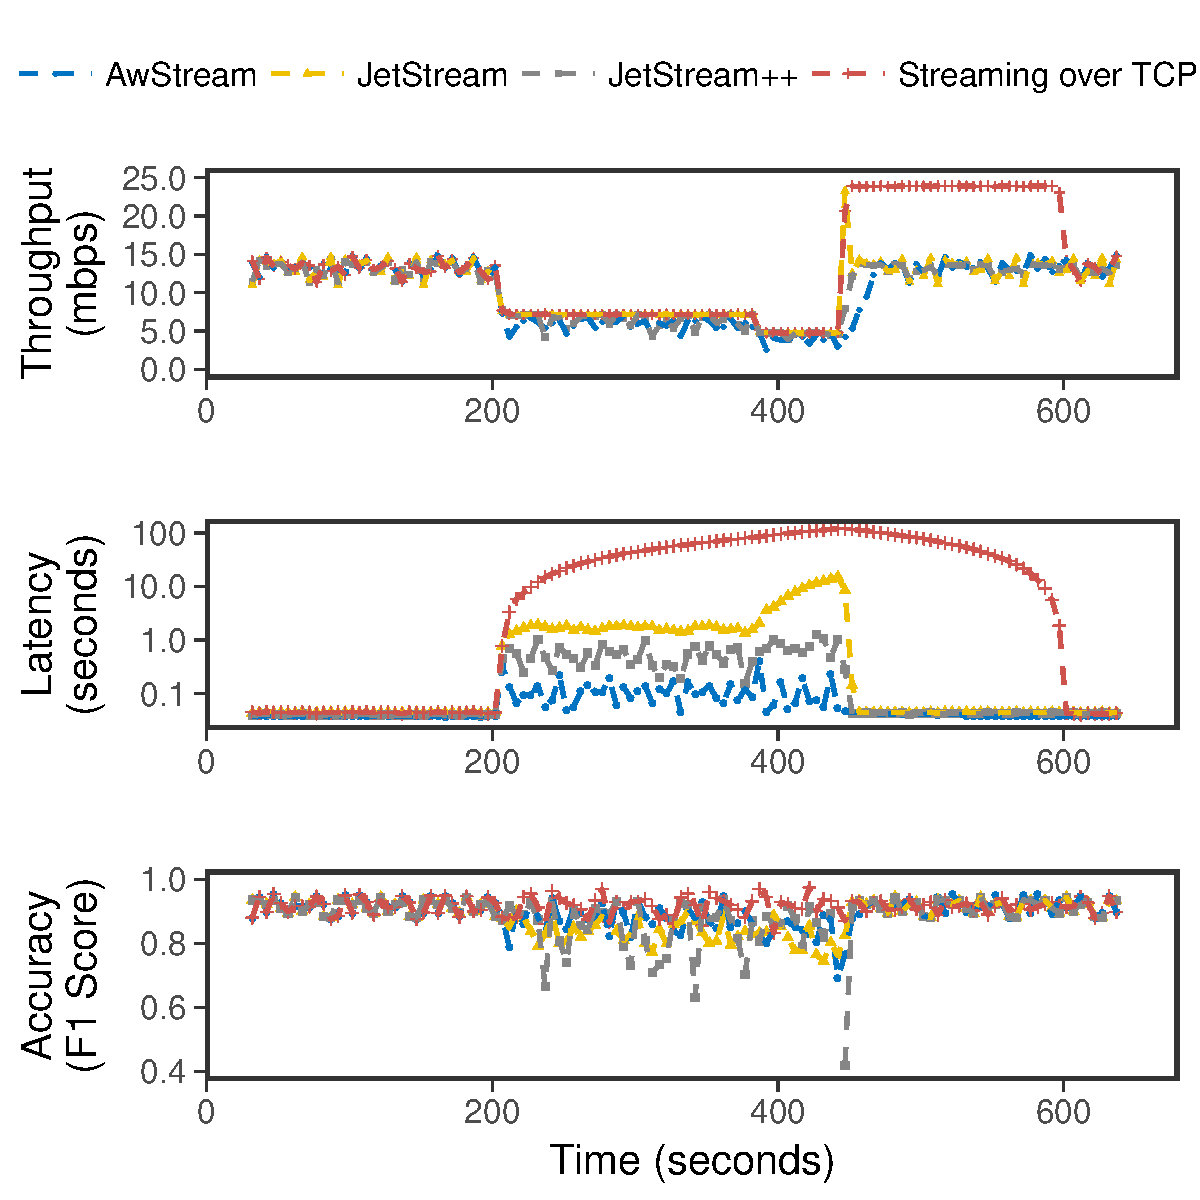
\includegraphics[width=\textwidth]{figures/runtime-darknet-verticle.pdf}
    \caption{Augmented Reality (AR)}
    \label{fig:ar-runtime}
  \end{subfigure}
  \hfill
  \begin{subfigure}{0.3\textwidth}
    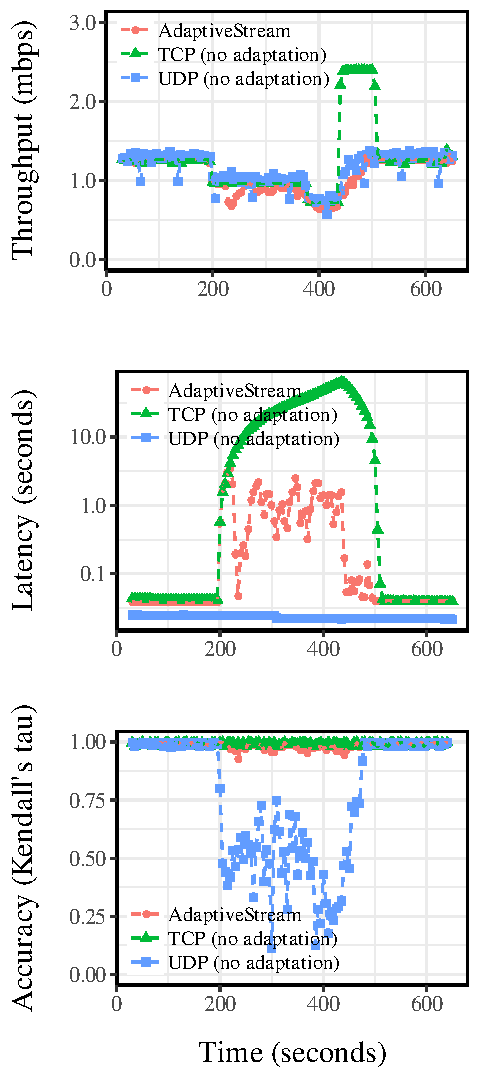
\includegraphics[width=\textwidth]{figures/runtime-topk-verticle.pdf}
    \caption{Top-K (TK)}
    \label{fig:tk-runtime}
  \end{subfigure}
  \caption{Runtime behavior of \sysname{} applications in comparison with streaming over TCP/UDP\@. AWStream simultaneously provides sub-second latency (similar to UDP) and high accuracy (similar to TCP).}
  \label{fig:all-runtime}
\end{figure*}

\newpage

\subsection{Runtime Adaptation}
\label{sec:runtime-adaptation}

In this section, we evaluate the runtime performance for three applications. We
first show that \sysname{} achieves low latency and high accuracy across all
three applications (\autoref{fig:all-runtime}).
We then focus on AR by evaluating how manual policies and
application-specific solutions work poorly, i.e., describe the experiments for
\autoref{fig:intro}.

We conduct our experiments on five geo-distributed machines from Amazon EC2,
spanning different AWS regions. Four act as worker nodes (\textit{t2.micro}
instances) and one acts as the aggregation server (\textit{m4.xlarge} instance
to guarantee enough bandwidth). During each experiment, the worker node
transmits test data (\autoref{tab:apps}) for about 10 mins. If the duration of
the test data is less than 10 mins, it loops.

We compare \sysname{} applications with baseline applications built with vanilla
TCP and UDP because they are universal for all applications. For streaming over
TCP, we use \sysname{} but disable the adaptation. For streaming over UDP, our
experiment setup is different: for video streaming (PD and AR), we use RTSP over
UDP with ffmpeg~\cite{bellard2012ffmpeg}; for TK, we implemented a simple
application protocol---packetization and a custom header---such that the receiver
can still aggregate data in the presence of UDP packet loss.

Because the baselines don't adapt the configuration and $B(c_{\max})$ is
prohibitively large---for example, raw videos consumes 230 mbps---we use a
reasonable configuration to limit the maximum rate. For PD, $c_{\max}$ is
1920x1080 resolution, \(10~\text{FPS}\) and a quantization of 20; it consumes about 12
mbps. For AR, $c_{\max}$ is 1600x900 resolution, \(30~\text{FPS}\) and a quantization of 20;
it consumes about 14 mbps.
For TK, $c_{\max}$ is $N=9750$ for \texttt{head} and $T=0$ for \texttt{threshold}.

Our controlled-experiment design follows JetStream~\cite{rabkin2014aggregation}. During
the experiment, we use the Linux \texttt{tc} utility with HTB~\cite{lartc,
  htb} to control the clients' outgoing bandwidth. Our experiments
involve four phases: (i) before t=200s, there is no shaping; (ii) at
t=200s, we start traffic shaping for 3 minutes (7.5 mbps for video
streaming and 1 mbps for TK); (iii) at t=380s, we further decrease the
available bandwidth (5 mbps for video streaming and 0.75 mbps) for TK);
(iv) at t=440s, we remove all traffic shaping. For UDP, HTB doesn't emulate the
packet loss or out-of-order delivery; we use \texttt{netem} and configure the
loss probability according to the delivery rate. Because different pair-wise
connections have different capacity, we impose a \textit{background} bandwidth
limit---25 mbps for PD and AR, 2.5 mbps for TK---to simplify comparisons.

The throughput figures of \autoref{fig:all-runtime} show the effect of our
traffic shaping. During the shaping, TCP and UDP make full use of the available
bandwidth; in comparison, \sysname{} is conservative. When we stop the shaping,
TCP has a ``catch-up'' phase where it's sending all the queued items as fast as
possible. \sysname{} increases the throughput gradually instead of drastically
as TCP/UDP does. This is when \sysname{} is slowly probing for more bandwidth.

The latency figures show that \sysname{} maintains a bounded latency. Note the
figures split in the middle because of the large variation in the measured
latency. Specifically, during the traffic shaping, TCP queues items at the
sender side for up to tens or hundreds of seconds. We plot such high latency
measurements in log scale. UDP always transmits as fast as possible, leading to
a consistent low latency. \sysname{}'s latency is slightly higher than UDP but
considerable small in comparison to TCP\@. During the traffic shaping,
\sysname{} controls the application's degradation to avoid data queueing up. For
most of the time, we've maintained less than 500 ms latency for PD/AR, and 2.5
seconds latency for TK\@. Because TK's source generates data every second after
the \texttt{window} operation, two objects in the queue would lead to two
seconds latency. The worst case happens at the start of bandwidth
drop: \sysname{} achieves sub-second latency for PD/AR and 5 seconds latency for
TK at the worst case.

The accuracy figures show that \sysname{} maintains a high accuracy throughout
the experiments. TCP without adaptation always sends data at high fidelity
(\textasciitilde 90\% for PD/AR and \textasciitilde 100\% for TK). It achieves
the high fidelity at the expense of increase latency. UDP without adaptation
suffers from packet loss, leading to a severe performance deterioration.  In
both PD and AR, the accuracy are \textasciitilde 0\% as the recovered images
contain large blocks of pixels without content details. For TK, the accuracy has
dropped to \textasciitilde 50\% during modest traffic shaping and dropped
further to \textasciitilde 25\% during the severe shaping. While \sysname{} also
sees an accuracy drop during the traffic shaping, the amount is significant
smaller: ~2\% drop on average in comparison to streaming over TCP\@.
We attribute this to the knowledge of the profile and the use of Pareto-optimal configurations during traffic shaping.

In summary, \autoref{fig:all-runtime} shows that \sysname{}'s adaptation achieves
low latency and high accuracy simultaneously.

\para{Fidelity and freshness.} Here we explain our experiments for
\autoref{fig:intro}. For streaming over TCP/UDP and \sysname{}, we use the
latency and accuracy measurements for AR\@. For manual policies, we implement the
policy from the example in JetStream~\cite{rabkin2014aggregation}. For
application-specific solutions, we apply PD's adaptation profile to control AR's
behavior.

For comparison, we use data collected during traffic shaping (between t=200s and
t=440s). When facing insufficient bandwidth, their behaviors reflect
the design choices within the design space of data fidelity and freshness:

\begin{itemize}[leftmargin=*]
\item Streaming over TCP favors fidelity over freshness.
\item Streaming over UDP favors freshness over fidelity.
\item Manual policies have limited rules with coarse-granularity. A sudden
  change from one rule to another incurs large latency (\textasciitilde 5
  seconds, similar to JetStream's result~\cite{rabkin2014aggregation}).
\item Application-specific solutions suffer from accuracy drop. PD's profile has
  configurations that reduce frame rate aggressively; these configurations work
  poorly for AR\@.
\item \sysname{} achieves both data fidelity and freshness.
\end{itemize}

\subsection{Resource Allocation and Fairness}
\label{sec:multi-task-alloc}

We evaluate resource allocations with two applications. In this way, the results
cover the case of a single application, and can generalize to more applications.

We choose PD and AR as the example applications.
We colocate the clients and servers of both applications so that they
share the same bottleneck link. The experiment starts with sufficient
bandwidth. At t=60s, we start traffic shaping to limit the total bandwidth
at 6 mbps. When we allocate resource equally between two applications
(\autoref{fig:eq-bw}), each application gets 3 mbps. Under this condition,
PD runs with a higher accuracy (\textasciitilde 85\%) while AR only achieves
\textasciitilde 77\%. In addition to resource fairness, \sysname{} supports utility fairness: it
chooses configurations that maximize the minimal accuracy. In this experiment,
PD receives 2 mbps and AR receives 4 mbps; and both achieve \textasciitilde 80\%
accuracy (\autoref{fig:eq-acc}).

\begin{figure}
  \begin{subfigure}[t]{0.9\columnwidth}
    \centering
    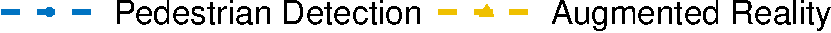
\includegraphics[width=\textwidth]{figures/multitask-legend.pdf}
  \end{subfigure}
  \\
  \vspace{1em}
  \begin{subfigure}[t]{0.49\columnwidth}
    \centering
    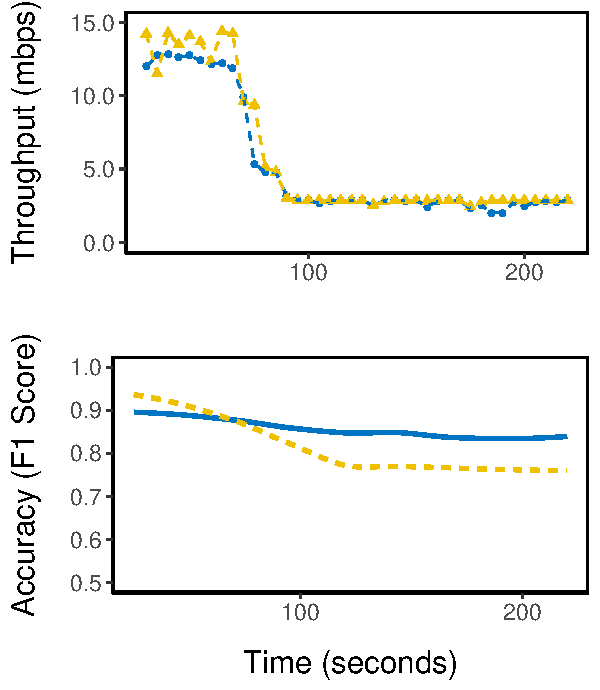
\includegraphics[width=\textwidth]{figures/multitask-eq-bw.pdf}
    \caption{Resource Fairness}
    \label{fig:eq-bw}
  \end{subfigure}
  \hfill
  \begin{subfigure}[t]{0.49\columnwidth}
    \centering
    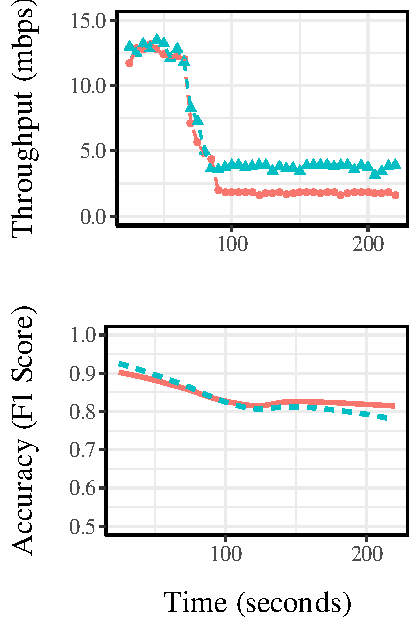
\includegraphics[width=\textwidth]{figures/multitask-eq-acc.pdf}
    \caption{Utility Fairness}
    \label{fig:eq-acc}
  \end{subfigure}
  \caption{\sysname{} supports a variety of resource allocation schemes (e.g., resource fairness and utility fairness).}
  \label{fig:multitask}
\end{figure}

%%% Local Variables:
%%% mode: latex
%%% TeX-master: "awstream"
%%% End:
